\chapter{Especificação do Sistema} \label{cap:especificacao}

A fim de realizar uma especificação do projeto completa e adequada frente ao contexto abordado e aos objetivos desejados, é proveitoso adotar um referencial teórico formal para orientar esse processo metodologicamente. Nesse sentido, o modelo adotado foi uma versão adaptada do \textit{Reference Model for Open Distributed Processing} (RM-ODP) \cite{tcc-rmodp}, o qual preconiza o estabelecimento de diferentes visões sobre o sistema de modo a separar as responsabilidades e melhor guiar o desenvolvimento. Além disso, essa alternativa se vale de um arcabouço teórico bastante conhecido e robusto e se aplica de forma conveniente para a modelagem do tipo de sistema e aplicação do projeto, o que a torna uma escolha propícia para o trabalho.

Mais especificamente, são propostas quatro visões:

\begin{itemize}
    \item \textbf{Visão Empresarial:} Contextualiza o sistema, o problema que pretende abordar, seus objetivos, atores/stakeholders e motivações para a aplicação.
    \item \textbf{Visão de Requisitos:} Elenca e detalha apropriadamente todos os requisitos do sistema (incluindo e diferenciando entre funcionais e não funcionais) e é alicerçada na Visão Empresarial.
    \item \textbf{Visão de Arquitetura:} Determina a estrutura do sistema, abarcando desde componentes individuais até grandes módulos e a forma como se conectam. Seu propósito é possibilitar e favorecer o atendimento da Visão de Requisitos.
    \item \textbf{Visão Tecnológica:} Delimita a implementação concreta do sistema, desde frameworks de software a serem empregados até quais componentes físicos serão utilizados. Sua meta é permitir que a Visão de Arquitetura seja posta em prática e efetivada cumprindo os requisitos impostos.
\end{itemize}

No projeto, essas visões ajudam a guiar a especificação e já se mostram presentes, visto que a Empresarial foi elaborada nos capítulos anteriores e as demais são discorridas no presente capítulo. Dito isso, vale ressaltar que esse modelo ainda será revisitado continuamente ao longo da execução do trabalho, permitindo aprimorar e aprofundar alguns tópicos e realizar eventuais modificações que venham a ser necessárias.

% ===================================================================
\section{Requisitos Funcionais}
% ===================================================================
 
Os requisitos funcionais descrevem as capacidades que o sistema, composto pelo
\textit{dongle} OBD-II e pelo \textit{companion app}, deve oferecer. Cada requisito recebe um identificador único (\texttt{RF-XX}), uma descrição objetiva e uma
prioridade (\palta, \pmedia{} ou \pbaixa).
 
\subsection{Dongle OBD-II}
 
\begin{longtable}{p{1.5cm} p{11cm} p{2cm}}
\caption{Requisitos Funcionais do Dongle OBD-II}
\label{tab:rf-dongle-cap-especificacao} \\
\toprule
\textbf{ID} & \textbf{Descrição} & \textbf{Prioridade} \\
\midrule
\endfirsthead

\toprule
\textbf{ID} & \textbf{Descrição} & \textbf{Prioridade} \\
\midrule
\endhead
 
RF-01 &
Ler parâmetros do veículo via protocolo OBD-II (PIDs padrão: rotação do motor,
velocidade, temperatura do líquido de arrefecimento e posição do acelerador). &
\palta \\ \hline
 
RF-02 &
Ler e retornar Diagnostic Trouble Codes (DTCs) armazenados na ECU do veículo. &
\palta \\ \hline
 
RF-03 &
Estabelecer comunicação sem fio (BLE ou Wi-Fi) com o \textit{companion app},
transmitindo os dados coletados em tempo real. &
\palta \\ \hline
 
RF-04 &
Exigir autenticação mútua com o \textit{companion app} antes de executar as funcionalidades de coleta e transmissão de dados. &
\palta \\ \hline
 
RF-05 &
Cifrar todo o tráfego transmitido sem fio entre o \textit{dongle} e o
\textit{companion app}. &
\palta \\ \hline
 
RF-06 &
Filtrar mensagens CAN enviadas ao barramento, permitindo somente mensagens
diagnósticas pré-definidas e rejeitando qualquer comando arbitrário. &
\pmedia \\ \hline
 
RF-08 &
Suportar atualização de firmware (\textit{over-the-air}) somente mediante
verificação de assinatura criptográfica, rejeitando pacotes inválidos. &
\pbaixa \\ \hline
 
RF-09 &
Entrar em modo de pareamento (aceitar nova conexão) apenas mediante acionamento
de botão físico no dispositivo, por período limitado de tempo. & \pmedia \\ \hline
 
RF-10 &
Expor uma interface de diagnóstico que permita consultar o estado de saúde interno
do \textit{dongle} (versão de firmware, status de conexão, contadores de erro). &
\pbaixa \\
 
\bottomrule
\end{longtable}

A prioridade alta foi dada às tarefas que exigem uma conexção direta com o hardware e estabelecimento do protocolo de comunicação, uma vez que esses aspectos são imprescindíveis para qualquer estudo de segurança no contexto do trabalhoe representam também a maior barreira de aprendizem para o começo da prototipação.

As prioridades média e baixa foram dada a atividades que, apesar de não serem essenciais para o trabalho, seriam interessantes de serem implementados para uma cobertura completa das vulnerabilidades estudades. Dentre eles, o requisito RF-08 recebeu prioridade baixa por ser a implementação mais difícil, podendo não se encaixar no tempo do projeto; e o requisito RF-10 pelo fato de representar apenas uma ajuda visual, não impactando diretamente o funcionamento de um MVP do projeto.
 
\subsection{Companion App}
 
\begin{longtable}{p{1.5cm} p{11cm} p{2cm}}
\caption{Requisitos Funcionais do Companion App}
\label{tab:rf-app-cap-especificacao} \\
\toprule
\textbf{ID} & \textbf{Descrição} & \textbf{Prioridade} \\
\midrule
\endfirsthead

\toprule
\textbf{ID} & \textbf{Descrição} & \textbf{Prioridade} \\
\midrule
\endhead
 
RF-11 &
Descobrir, parear e conectar-se ao \textit{dongle} OBD-II de forma segura,
utilizando o protocolo de autenticação definido na arquitetura. &
\palta \\ \hline
 
RF-12 &
Exibir em tempo real os parâmetros lidos do veículo (PIDs) em telas de
visualização claras e navegáveis. &
\palta \\ \hline
 
RF-13 &
Apresentar e interpretar DTCs retornados pelo \textit{dongle}, informando ao
usuário o significado de cada código. &
\pmedia \\ \hline
 
RF-14 &
Exibir o histórico de leituras de odômetro recuperado do \textit{dongle},
alertando o usuário caso seja detectada inconsistência ou indício de adulteração. &
\pbaixa \\ \hline
 
RF-15 &
Conduzir o usuário pelo processo de pareamento via botão físico (RF-09),
orientando cada etapa por meio de instruções na interface. &
\pbaixa \\ \hline
 
RF-16 &
Permitir a exportação dos dados coletados em
formato aberto (CSV ou JSON) para uso externo. &
\pbaixa \\
 
\bottomrule
\end{longtable}

Na implementação do \textit{companion app}, foi dada prioridade alta para os elementos diretamente relacionados ao estudo de segurança, ou seja, pareamento e comunicação do \textit{dongle}.

O requisito RF-13 recebeu prioridade média pelo fato de, mesmo não sendo essencial para o trabalho a visualização de DTCs, a garantia de sua integridade é importante para garantir que nenhum atacante esteja influenciando na manutenção do veículo, ou seja, ainda representar um aspecto de segurança.

Os outros requisitos recebem prioridade baixa por não estarem relacionados com segurança.

 
% ===================================================================
\section{Requisitos Não Funcionais}
% ===================================================================
 
Os requisitos não funcionais estabelecem restrições de qualidade, desempenho,
segurança e conformidade que o sistema deve satisfazer. Cada requisito recebe um
identificador (\texttt{RNF-XX}) e uma prioridade.


\begin{longtable}{p{1.5cm} p{11cm} p{2cm}}
\caption{Requisitos Não-Funcionais do Sistema}
\label{tab:rnf-sistema-cap-especificacao} \\
\toprule
\textbf{ID} & \textbf{Descrição} & \textbf{Prioridade} \\
\midrule
\endfirsthead

\toprule
\textbf{ID} & \textbf{Descrição} & \textbf{Prioridade} \\
\midrule
\endhead

RNF-01 & 
Os dados transmitidos via interface sem fio devem ser protegidos por mecanismos de cifração que garantam a confidencialidade e integridade das informações. & 
\palta \\ \hline

RNF-02 & 
O sistema deve utilizar métodos de autenticação robustos para garantir que apenas dispositivos autorizados estabeleçam conexão com o hardware. & 
\palta \\ \hline

RNF-03 & 
O processo de atualização de firmware deve incluir mecanismos de verificação de origem e integridade para impedir a execução de código não autorizado. & 
\palta \\ \hline

RNF-04 & 
O sistema deve ser validado contra as principais vulnerabilidades de segurança documentadas na literatura para dispositivos de diagnóstico automotivo. & 
\palta \\ \hline

RNF-05 & 
O dispositivo deve operar em conformidade com as normas e padrões internacionais de diagnóstico veicular (ISO 15765-4 e SAE J1979). & 
\palta \\ \hline

RNF-06 & 
A latência de comunicação entre a coleta de dados no barramento e a visualização no aplicativo deve ser compatível com o monitoramento em tempo real. & 
\pmedia \\ \hline

RNF-07 & 
O sistema deve garantir a estabilidade da conexão sem fio e possuir mecanismos de recuperação automática em caso de desconexão momentânea. & 
\pmedia \\ \hline

RNF-08 & 
O software do aplicativo deve ser compatível com as versões atuais dos sistemas operacionais móveis predominantes no mercado. & 
\pmedia \\ \hline

RNF-09 & 
A arquitetura e o software elaborados, especialmente no que diz respeito ao dongle, devem ser compatíveis com dispositivo embarcado de baixo poder computacional. & 
\pmedia \\ \hline

RNF-10 & 
A arquitetura de software deve ser modular, seguindo boas práticas de desenvolvimento e padrões de projeto. & 
\pmedia \\ \hline

RNF-11 & 
A interface do usuário deve ser intuitiva, permitindo o acesso às funcionalidades principais com o mínimo de intervenção manual. & 
\pbaixa \\ 

\bottomrule
\end{longtable}

Nos requisitos não funcionais, recebem prioridade alta os requisitos relacionados a segurança, prioridade média os requisitos não relacionados a segurança que garantem a utilização do sistema seja confiável e compatível (RNF-06, RNF-07 e RNF-08), ou que estejam em linha com as contribuições do projeto (RNF-09 favorece reprodutibilidade e um projeto final mais econômico em termos financeiros e de uso de recursos, ao passo que RNF-10 também facilita reprodutibilidade e manutenção de base de código \textit{open source}).

\section{Arquitetura}


A arquitetura proposta para este trabalho foi concebida sob o princípio da modularidade. O sistema é segmentado em três domínios principais: a Camada Veicular, o Dongle OBD-II Seguro e o Companion App.

\subsection{Visão Geral e Fluxo de Dados}

O fluxo de informações inicia-se na Camada Veicular, onde os dados de diagnóstico são extraídos do barramento CAN através da porta física OBD-II \cite{csselectronics_obd2_intro}. O Dongle atua como uma ponte controlada, processando as requisições do usuário e aplicando políticas de filtragem \cite{wen2020plugnpwned}. Por fim, o Companion App funciona como a interface de controle e autenticação \cite{companionapps2024security}. A \autoref{fig:arquitetura-preliminar-cap-especificacao} exibe uma visão geral da arquitetura proposta.

\begin{figure}[H]
    \centering
    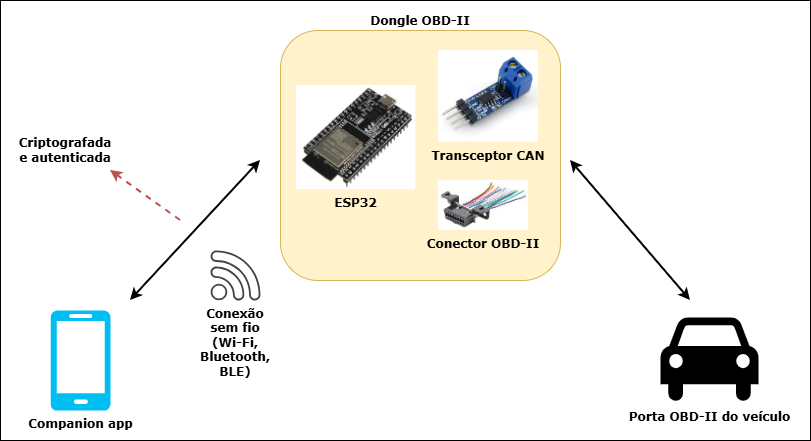
\includegraphics[width=0.9\linewidth]{assets/cap4-especificacao/arquitetura-preliminar.png}
    \caption{Arquitetura geral proposta para o sistema}
    \label{fig:arquitetura-preliminar-cap-especificacao}
\end{figure}

\subsection{Módulos do Dongle OBD-II}

O hardware é organizado em blocos lógicos, os quais incluem tanto componentes físicos quanto de software:

\begin{itemize}
    \item \textbf{Interface CAN:} Responsável pela sinalização física segundo o padrão ISO 15765-4 \cite{malekian2017fleet}.
    \item \textbf{Comunicação Sem Fio:} Permite que o sistema opere via Bluetooth ou Wi-Fi \cite{wen2020plugnpwned}.
    \item \textbf{Módulo de Segurança:} Centraliza as primitivas criptográficas para cifração e autenticação \cite{companionapps2024security}.
    \item \textbf{Filtro de Mensagens (Allow-list):} Atua como um \textit{firewall} para o barramento CAN, impedindo a injeção de comandos arbitrários \cite{wen2020plugnpwned}.
\end{itemize}

Do ponto de vista físico, o hardware tem como seu elemento central o microcontrolador ESP32, o qual consiste em um dispositivo acessível, com um poder computacional relativamente baixo (típico para aplicações embarcadas de borda) e que, ainda assim, conta com uma variedade de recursos oportunos, como módulos de comunicação sem fio (Wi-Fi e Bluetooth/BLE) e um controlador CAN embutido \cite{esp32-datasheet}. Assim, a placa fica responsável por efetivar a intermediação da comunicação entre o app e o veículo, implementando regras de negócio e mecanismos de segurança.

Para que um dispositivo possa se conectar a uma rede CAN, são necessários dois componentes especializados \cite{can_standard_overview}: um controlador CAN, responsável por implementar o protocolo lógico do enlace de dados, e um transceptor CAN, responsável por realizar as conversões de sinais para os formatos adequados de cada camada física. A \autoref{fig:can-conexao-cap-especificacao} ilustra esse esquema e suas interfaces.

\begin{figure}[H]
    \centering
    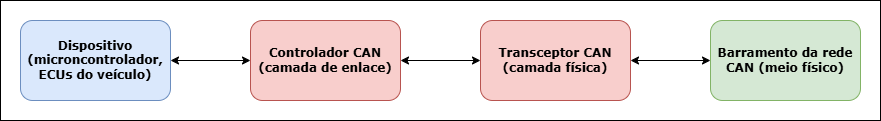
\includegraphics[width=0.9\linewidth]{assets/cap4-especificacao/conexao-can.png}
    \caption{Esquema geral de um nó de rede CAN}
    \label{fig:can-conexao-cap-especificacao}
\end{figure}

Desse modo, para possibilitar toda a comunicação do projeto, serão utilizados mais dois elementos: o transceptor CAN mencionado - a exemplo do SN65HVD230 \cite{SN65HVD23x-datasheet} - e um conector OBD-II para interfaceamento com a porta localizada no veículo, compondo assim o esquema da \autoref{fig:arquitetura-preliminar-cap-especificacao}.

\subsection{Arquitetura do Companion App}

O aplicativo móvel é estruturado para espelhar as garantias de segurança do hardware \cite{companionapps2024security}:

\begin{itemize}
    \item \textbf{Gerenciador de Conexão:} Responsável pela descoberta e link sem fio.
    \item \textbf{Núcleo de Cifração e Autenticação:} Utiliza armazenamento seguro como o Android Keystore \cite{companionapps2024security}.
    \item \textbf{Interpretador de Protocolo:} Realiza a tradução das respostas brutas do dongle.
\end{itemize}

\subsection{Modelo de Confiança e Comunicação Segura}

O sistema adota um modelo de segurança baseado na proximidade física para o pareamento inicial entre dongle e app \cite{wen2020plugnpwned}. A comunicação subsequente utiliza um esquema criptográfico para garantir a confidencialidade, integridade e autenticidade dos dados \cite{companionapps2024security}, o qual consiste essencialmente no uso inicial do ECDH como método assimétrico para obtenção de uma chave privada compartilhada e no uso do AES-GCM para cifração e autenticação simétricas das mensagens trocadas.
